\chapter{Characterisation and operation of the microscope}
\label{chap:characterisation}

This appendix gives more details on the optics of the microscope, with a focus on the polarisation state of light at different points in the beam paths. These are important for operating the setup, but less so for understanding the project as a whole.

\section{The laser modules}

The fast-switching 561~nm laser emits horizontally polarised light, but the polarisation can be tuned by three waveplates in its path. The last one, a quarter-wave plate, is fixed in its rotation angle. In the standard mode of operation, excitation laser light should be circularly polarised to minimise resolution reduction due to lens distortion etc.~\cite{Harke2008}. In that mode, the (fast or slow) axis of the first quarter-wave plate is aligned with the laser, such that it does not affect polarisation and the half-wave plate is set such that it rotates the (linearly polarised) light to \ang{45} with respect to the second quarter-wave plate. See \autoref{tab:laser polarisation} for the polarisation characteristics in the calibration provided by Abberior. The 561~nm laser is quite well-calibrated. In circular polarisation, it reaches a $ \chi$ very close to perfectly circular (\ang{45}).

The 640 nm laser does not have fast-switching built in, so instead, the light is fed into the microscope through a polarisation-preserving optical fibre by an acousto-optical modulator (AOM). The AOM is a crystal in the beam path, in which sound waves can be generated by a piezo element. The standing sound wave creates a diffraction grating with a variable pitch. That pitch is determined by the sound frequency, which can be modulated such that the first-order diffracted beam is either sent into the fibre aperture or not. The rest of the beam path is very similar to the 561 module, but the calibration of the waveplates in this pathway is not as accurate. Refer to \autoref{tab:laser polarisation}. 

The depletion laser travels through an entirely different set of optics than the excitation lasers to generate a donut beam. First, it travels through a half-wave plate that aligns the polarisation to the SLM (spatial light modulator). This HWP is necessary because an SLM adds an arbitrary spatially patterned phase delay to incident light, but only to the component polarised along its active axis. It will not alter the phase of the orthogonally polarised component. Using the proper phase delay patterns, one can create any (diffraction-limited) image in the sample plane. In this case, that would be a donut shape. Then -- ignoring the pSTED module for now, since that was not included in the original setup -- the beam travels through a half-wave plate to ensure circular polarisation in the sample plane (after going through a quarter-wave plate at \ang{45} to the QWP axes), just like the excitation lasers. This is done to ensure that the depletion efficiency does not depend on sample orientation and to avoid polarisation-dependent PSF distortion by lenses and other optics. The quality of the STED polarisation is similar to that of the 640 nm laser. Note that this is actually a significant result, since it means that the donut beam is not isotropically polarised. It will be far more effective at quenching fluorophores oriented along \ang{40} than those at \ang{130}.

\begin{table}
	\centering
	\begin{tabular}{lSSSS}
		\toprule
		Laser source     & {$ I_\mathit{max} / I_\mathit{min} $} & {$ \chi_I$ (deg)} & {$ \chi_E $ (deg)} & {$ \psi$ (deg)} \\ \midrule
		561 nm, linear (\ang{0})  & 23.6                              & 2.42                               & 11.6                               & 0                                \\
		561 nm, circular & 1.14                              & 41.2                               & 43.1                               & 20                               \\
		640 nm, linear (\ang{0})  & 6.13                              & 9.25                               & 22.0                               & 0                                \\
		640 nm, circular & 1.59                              & 32.2                               & 38.5                               & 120                              \\
		775 nm, circular & 1.61                              & 31.8                               & 39.2                               & 40                               \\ 
		775 nm, linear & 5.47 & 10.6 & 23.1 & 0 \\ \bottomrule
	\end{tabular}
	\caption{
		Polarisation characteristics of the lasers. Shown are linearity $ I_\mathit{max} / I_\mathit{min} $, ellipticity $ \chi_E $ ($ \chi_I$) of the electric field (intensity), and ellipse orientation $ \psi$ (anti-clockwise angle between ellipse orientation and vertical axis in sample plane). This data is based on \autoref{fig:laser polarisation}, except the linear setting of the 775 nm laser. This required fitting new waveplates, as explained later (\autoref{sec:psted implementation}).
	}
	\label{tab:laser polarisation}
\end{table}

\begin{figure}
	\centering
	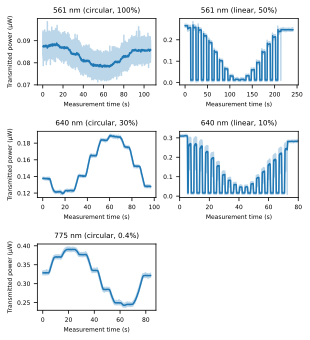
\includegraphics{laser_polarisation}
	\caption{
		Polarisation characterisation of the different lasers. To characterise circular polarisation, a polariser was placed in the sample and scanned from \ang{0} to \ang{180} in steps of \ang{20} (note that a sample is lacking at \ang{260} in the 775 nm data). Linear polarisation was characterised by fixing the polariser in place at \ang{0} and scanning the laser itself from \ang{0} to \ang{180} in steps of \ang{10}. Dark blue: average over 200 samples, light blue: raw data.
	}
	\label{fig:laser polarisation}
\end{figure}

One more thing we can derive from this data (see \autoref{fig:laser polarisation}), is that the 640 laser needs to ramp up every time it is powered on, due to the lack of fast switching.
This can be somewhat remedied in software by turning the laser ``on'', but at 0\% power. The effect of this is that the laser is on but the AOM directs laser light away from the fiber aperture, thereby shortening the time to ramp up the laser power. Furthermore, at low powers, the laser intensity may not be proportional to the power setting in software. Their actual relationship is shown in \autoref{fig:laser power}. If experiments need to be done at low power, a neutral density filter is required. This is luckily not the case for biological specimens with a low density of fluorophores.

\begin{figure}[ht]
	\centering
	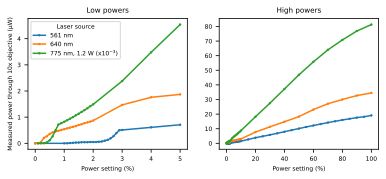
\includegraphics{laser_power}
	\caption{
		The power of each of the three lasers as measured through a 10x objective. Notice the non-linearity at low power settings. The 775 nm data was scaled down by three orders of magnitude.
	}
	\label{fig:laser power}
\end{figure}

Looking at the calibrations of the waveplates in the excitation modules (\autoref{fig:excitation waveplate calibration}), one can see that they move quite erratically, but they do work, as shown in \autoref{fig:laser polarisation}. This could be an effect of the automated calibration performed by Abberior. In the 561 nm calibration, for example, one can see that the QWP constantly flips between about \ang{30} and \ang{120}, which are \ang{90} apart. The calibration works, but the eccentricity of the polarisation ellipse depends on the orientation. In other words, for a more rigorous characterisation of the microscope, \autoref{tab:laser polarisation} should have an entry for every possible calibration setting.

\begin{figure}
	\centering
	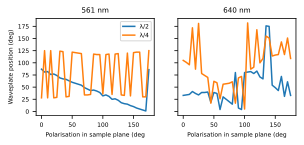
\includegraphics{excitation_waveplate_calibrations.pdf}
	\caption{
		Calibrations of the excitation waveplates, as supplied by the microscope manufacturer.
	}
	\label{fig:excitation waveplate calibration}
\end{figure}

One can measure the PSFs of the lasers by scanning over a reflective gold bead and acquiring an image on the photomultiplier tube (PMT). These are shown in \autoref{fig:normal psfs}.

\begin{figure}
	\centering
	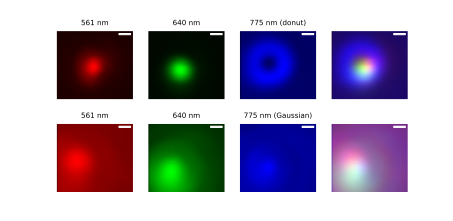
\includegraphics{laser_psfs.pdf}
	\caption{
		Point spread functions of the different lasers (in donut and Gaussian modes) at different SLM configurations, by measuring the reflection from 100 nm wide gold beads.
	}
	\label{fig:normal psfs}
\end{figure}

\section{The detection module}

The main detectors of the microscope are a set of avalanche photodiodes (APDs), but there is also a highly sensitive PMT right after the QWP on the microscope end. The PMT is usually used to measure the point spread functions of the lasers and to align them with each other. In normal operation, the light travels on to the detection waveplates, then through a pinhole wheel, passes filters and dichroic mirrors in the filter cube housings, and is finally reflected onto the APDs. The wheel contains pinholes of different sizes, which allows for choosing the trade-off between light collection and $ z $ resolution, depending on the quality of the sample. Different filter cubes are available with various bandpass filters, dichroic mirrors, and/or a polarising beam splitter (PBS).

The APDs show a slight polarisation sensitivity of about 10\% (see \autoref{fig:apd pol sensitivity}). I measured this by exciting Tetraspec beads with the 561 laser set to circular excitation, such that the emission light is non-polarised. Then I placed a linear polariser behind the detection waveplates and measured their signal as a function of the polariser angle. It seemed like the beam moved depending on the incident polarisation, as aligning the APDs when the signal was minimal did help a little, but the imperfect circularity of the 561 laser may also play a role, as it is on the same order of magnitude. 

\begin{figure}
	\centering
	\includegraphics{apd_pol_sensitivity.pdf}
	\caption{Dependence of the signal from APD1 on the angle of polarisation of incoming light.}
	\label{fig:apd pol sensitivity}
\end{figure}

\subsection{Calibrating the detection waveplates}

We did have some problems with the waveplates in the detection module. They can be controlled through Abberior's software suite (Imspector), but it is not clear if they are set up correctly. The calibration is based on a control angle that I will denote $ \theta $. It would theoretically be possible for this setup to rotate polarised light of any orientation, since
\begin{equation}
	S_\hwp(\theta/2) S_\qwp(0) S_\qwp(0) = \mqty(\cos\theta & -\sin\theta \\ \sin\theta & \cos\theta ),
	\label{eq:detection waveplates}
\end{equation}
which is simply the rotation matrix $ R(\theta) $. The exact position of the quarter-wave plates does not matter, as long as they are aligned with each other. If the waveplates are at an angle $ \phi$ instead of 0, then this set of waveplates rotates the polarisation by an angle $ (\theta-2\phi) $ instead. 

It is unclear what goal the original calibration (see \autoref{fig:detection waveplate calibrations}) should serve. If we approximate the default calibration with a QWP at $ \theta $ and a HWP at 0, then the action of these waveplates would be
\begin{equation}
	S_\hwp(0)\cdot S_\qwp(\theta)\cdot S_\qwp(0) = 
		\mqty( \cos^2\theta + i\sin^2\theta & (1+i)\cos\theta\sin\theta \\
			   (-1+i)\cos\theta\sin\theta   & \cos^2\theta - i\sin^2\theta 
	    ).
\end{equation}

Therefore, I developed a new calibration. To do so, I first needed to establish at what angle the second quarter-wave plate would be aligned to the first one. I did this by placing a polariser in the sample holder (P1) and illuminating it with the top lamp, such that the light incident on the first quarter-wave plate was linearly polarised. Then I placed another polariser (P2) after that waveplate (i.e.~before the last two waveplates) that I rotated to assess the linearity of the polarisation there. I found the angle of P1 at which light was most circular after the first QWP and subsequently placed P2 after all waveplates to find the angle of the second QWP that would make the polarisation linear again. At this point, the QWPs should be aligned. They could also be at \ang{90} to one another. To distinguish between these setups, compare a measurement such as \autoref{fig:p1 effects} with simulations in \autoref{fig:detection waveplate simulations}.

\begin{figure}
	\centering
	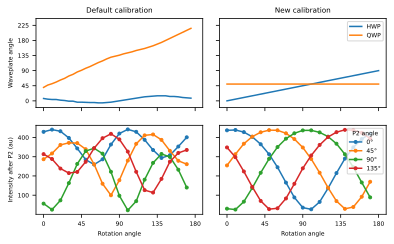
\includegraphics{detection_waveplate_calibrations.pdf}
	\caption{
		A comparison of the default detection waveplate calibration and the new one. The new calibration seems to actually rotate incident polarisation by an arbitrary angle.
	}
	\label{fig:detection waveplate calibrations}
\end{figure}


\begin{figure}
	\centering
	\includegraphics[scale=.95]{p1_effects_qwp_aligned.pdf}
	\includegraphics[scale=.95]{p1_effects_qwp_30.pdf}
	\includegraphics[scale=.95]{p1_effects_qwp_90.pdf}
	\caption{
		Simulation of the effect of QWP alignment on the action of the detection pathway. Shown are three simulations in which the first QWP is rotated by 0, 30, and 90 degrees, respectively. The second QWP is always rotated by 0, and the HWP is rotated to half the rotation angle (x-axis). When the QWPs have an offset of 90 degrees (bottom), the upper and lower panels (with either P1 or P2 constant) are identical, but when they are aligned (top), there is a phase difference. When they are not aligned at all (middle), intensity variations are prominent. This simulation is based on \autoref{eq:detection waveplates}.
	}
	\label{fig:detection waveplate simulations}
\end{figure}


Second, I assessed both calibrations. As presented in \autoref{fig:detection waveplate calibrations}, the new calibration works rather well, unlike the original one. However, its performance seems to depend on the precise angle of P1, see \autoref{fig:p1 effects}.
This needs to be fixed before we can confidently use polarisation-affecting elements in the detection path. Luckily, simulations show that this effect can be explained by misalignment between the QWPs. Therefore, a more accurate calibration should fix this problem.

\begin{figure}[h]
	\centering
	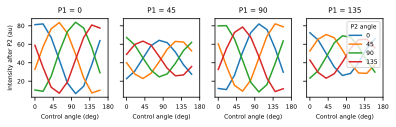
\includegraphics{p1_effects.pdf}
	\caption{
		The effect of rotating the incoming polarisation (P1). The detection waveplates seem to rotate the polarisation for P1 at \ang{45} or \ang{135}, but seem to circularise incoming light at \ang{0} and \ang{90} somewhat. (Note that the angle of P1 does not have a proper reference since I forgot to home the rotator.)
	}
	\label{fig:p1 effects}
\end{figure}


Finally, I checked the POL cube, which contains a polarising beam splitter (PBS) and some wavelength filters. It seems to work as expected (see \autoref{fig:pol cube}). The transmitted ray has an extinction ratio of about 0.2, meaning that 20\% of the power of rays that are orthogonally polarised to the transmission axis (and hence should be reflected by the PBS) is actually transmitted. On the other hand, it has an extinction ratio of .01 for the reflected wave.

\begin{figure}
	\centering
	\includegraphics{pol_cube.pdf}
	\caption{Performance of the polarising beam splitter.}
	\label{fig:pol cube}
\end{figure}

\section{Protocol for polarisation microscopy}
\label{sec:polarisation microsocpy protocol}

After acquisition, a stack of images $ I_{nxy} $ (with excitation light polarised along $ \theta_n $) must go through a number of steps to be converted into a false-colour polarisation image. Those steps are detailed in this section.

\subsection{Stack alignment.} Images in a stack are aligned using an ECC (enhanced correlation coefficient) optimisation algorithm implemented in OpenCV, an open source computer vision library, which optimises an adjusted version of the correlation between two images, subject to certain constraints, e.g.~translation, without shearing or rotation \cite{Evangelidis2008}. When the correlation between two images is maximised, they are aligned. The innovation of the ECC algorithm lies in the definition of an enhanced correlation coefficient which requires less computational power and is more robust than other algorithms \cite{Evangelidis2008}. 

If the goal is to generate a new image stack $ I'_{nxy} $, corrected for sample or beam drift, we can take the first frame as reference, setting 
\begin{equation}
	I'_{0xy} = I_{0xy}.
\end{equation}
For every other frame $ I_{nxy} $, we can calculate a warp matrix using OpenCV with the \texttt{findTransformECC()} method, which maximises the correlation between $ I_{nxy} $ and $ I'_{(n-1)xy} $. Since we only observe drift in the images, we only allow translation (no shearing or rotation). Finally, we transform the original image using that warp matrix and \texttt{warpAffine()} and save the result as $ I'_{nxy} $.

\noindent In other words:
\begin{equation}
	I'_{nxy} = \texttt{warpAffine}\left(
		I_{nxy},\,
		\texttt{findTransformECC}\left(I'_{(n-1)xy}, I_{nxy}\right)
	\right),
\end{equation}
for all $ n>0 $.

\subsection{Bleaching compensation.} Since photobleaching will influence the calculation of the Fourier coefficients, it needs to be separated from the polarisation response. We can estimate the bleaching rate from the ratio between two frames at identical polarisations. Unfortunately, the Imspector software suite does not allow for rotating the excitation polarisation by more than \ang{175}, so we cannot do this exactly. It would be possible if we were able to use the POL cube, but that is not an option, as explained before. Let $ \bar{I}_0 $ be the mean intensity of the first image, and $ \bar{I}_N $ the mean intensity of the last one. For now, we simply estimate the bleaching per frame as
\begin{equation}
	r = \left( \frac{\bar{I}_N}{\bar{I}_0} \right) ^{1/N},
\end{equation}
given $ N+1 $ number of frames were acquired. Then we can compensate for photobleaching by multiplying every frame with a correction factor as
\begin{equation}
	I''_{nxy} = r^{-n} I'_{nxy}.
\end{equation}

\subsection{Colouring the image.} For every pixel, calculate a complex-valued Fourier coefficient corresponding to a period of \ang{180} (at which we should see polarisation dependence) using
\begin{align}
	F_{xy} &= \sum_n I''_{nxy} e^{i2\theta_n}.
\end{align}
Then construct an image in HSV colour space where 
\begin{align}
	h_{xy} &= \arg (F_{xy}),\\
	s_{xy} &= \abs{F_{xy}}/v_{xy},\\
	v_{xy} &= \sum_n I_{nxy}.
\end{align}
Finally, normalise every channel $ c $ to be in the range $ (0,1) $ and optionally apply a power law with a manually chosen coefficient $ \alpha_c $ for optimal visualisation,
\begin{equation}
	c'_{xy} = \left( \frac{c_{xy}}{\max c_{xy}} \right)^{\alpha_c}.
\end{equation}
The effect of $ \alpha_c $ is presented in \autoref{sec:conventional pol}. If necessary, the Fourier image $ F_{xy} $ can be blurred before constructing a false colour image. This can be useful when the image is too noisy for a decent Fourier calculation.

\section{pSTED optics}

\label{sec:psted implementation}

The system was not set up to offer control over the depletion polarisation. Instead, the STED polarisation is always circular, and this is ensured by a set of two fixed waveplates: a QWP and a HWP (refer to \autoref{fig:layout} and the description of the STED module in that section). 

To control the polarisation of the depletion beam for pSTED, I first had to linearise the polarisation by compensating for the QWP in the beam path. That can be done by placing a QWP in the pSTED module in \autoref{fig:layout}, since
\begin{equation}
	S_\qwp(\phi)S_\hwp(0)S_\qwp(-\phi) = R(2\phi).
\end{equation}
When the quarter-wave plates are aligned like that (when they are each others mirror image with respect to the HWP fast axis), this system simply rotates the polarisation by a fixed angle. This means that adding a HWP before this setup suffices to get full control over the polarisation angle of the depletion beam.

\begin{figure}
	\centering
	\includegraphics[height=.35\linewidth]{psted optics 1.jpg}%
	\hfill%
	\includegraphics[height=.35\linewidth]{psted optics top.jpg}
	\caption{
		The new pSTED optics. The rotational stage holds a HWP and a stationary QWP is mounted on a cage system. To take these optics out of the microscope, only the screw that holds the foot needs to be removed.
	}
	\label{fig:psted optics photo}
\end{figure}

In practice, the first step was to mount these two new waveplates in the beam path. They were mounted right after the SLM on an easily removable foot, see \autoref{fig:psted optics photo}. This way, conventional STED and polarisation-dependent STED are both easily performed. The HWP was mounted inside a rotational stage and the QWP in a cage system attached to the rotational stage, such that it is always aligned with the laser beam, but that its rotational angle is fixed. The first step was to find the angle of the QWP that maximised the linearity of the light polarisation at the sample. This was done by placing a polariser and a power meter at the sample and rotating them to characterise the polarisation of the depletion beam. I did this a couple of times, from which we concluded that the optimal angle for the QWP was \ang{15}. Next, I had to find the angle of the HWP at which the depletion beam is vertically polarised. In that position, the depletion beam has a polarisation parallel to the excitation lasers (at \ang{0}). This turned out to be \ang{38.5} (or equivalently $\ang{38.5}+\ang{180}=\ang{218.5}$). See \autoref{fig:psted hwp offset}. At a linearity of $ I_{max}/I_{min} = 5.47 $, the polarisation of the linearised pSTED beam is comparable in quality to the 640 laser (see \autoref{tab:laser polarisation}). Note that the HWP angle $ \theta_\hwp $ must satisfy
\begin{equation}
	\theta_\hwp = \ang{218.5} - \theta/2
\end{equation} 
to achieve a linear polarisation along $ \theta $ in the sample plane.

\begin{figure}
	\centering
	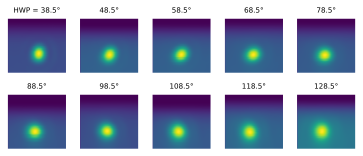
\includegraphics{psted_psfs.pdf}
	\caption{
		Depletion PSF as a function of beam polarisation. The figure titles indicate the angle of the new HWP. The shown images are recentred on the pixel with the highest intensity to correct for displacement.
	}
	\label{fig:psted psfs}
\end{figure}

Now that we have control over the beam polarisation, we can check how the new waveplates influence the PSF. In \autoref{fig:psted psfs}, the PSF is shown for different polarisation directions. There are several conclusions we can draw from this data.  Firstly, the PSF is not radially symmetric any longer, even though the SLM was set to Gaussian mode. (This is easy to do. It only requires removing the donut-generating pattern on the SLM.) In particular, the ellipse orientation is parallel to the light polarisation, so we see the PSF rotating as we change the polarisation (see also \autoref{fig:psted psf orientation and power}). This can be explained by the fact that lenses interacts differently with light polarised along different directions \cite{Egner2020}. This is the reason one should only use linearly polarised excitation light when performing polarisation microscopy.

Other effects of the polarisation include the following: the intensity of the depletion beam varies as a function of the polarisation angle (see \autoref{fig:psted psf orientation and power}). This is probably due to linear dichroism present in the optical elements between the waveplates and the sample. This is not a surprising result, but should be accounted for during either image acquisition or analysis. Furthermore, the maximum of the PSF moves a little: up to roughly 100~nm from its mean position (\autoref{fig:psted displacement}). Fortunately, this is quite a bit below the diffraction limit for 775 nm light, i.e.~around 400 nm, so the effect will be rather small.

\begin{figure}
	\centering
	\includegraphics{psted_hwp_offset.pdf}
	\caption{
		The new rotating HWP in the pSTED module controls the depletion beam polarisation. With an offset of 38.5°, the depletion beam is parallel to the 640 laser (set to vertical linear polarisation).
	}
	\label{fig:psted hwp offset}
\end{figure}

\begin{figure}
	\centering
	\includegraphics{psted_psfs_orientation_and_power.pdf}
	\caption{
		\textbf{Left:} The pSTED PSF is elliptical, and its orientation matches the light polarisation. \textbf{Right:} pSTED intensity depends on polarisation. Error bars show standard deviation, n=10.
	}
	\label{fig:psted psf orientation and power}
\end{figure}

\begin{figure}
	\centering
	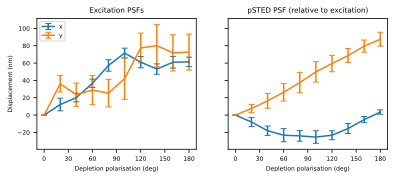
\includegraphics{psted_psfs_displacement.pdf}
	\caption{
		The displacement of the laser PSFs as a function of depletion polarisation. \textbf{Left:} The displacement of the 561~nm and 640~nm PSFs (representing drift in the image). \textbf{Right:} Displacement of the pSTED PSF relative to the excitation PSFs.
	}
	\label{fig:psted displacement}
\end{figure}